%
% File          : 5GAKA-proof.tex
% Description   : 5G-AKA Proof Paper
% Authors       : Clayton & Harmon
%
% Last Modified : Fri Dec  1 08:17:28 EST 2000
%
% BDOC PARAM offset=0in,0in

% Page style
\documentclass[11pt, pdftex]{article}
\usepackage{epsf}
\usepackage{epsfig}
\usepackage{times}
\usepackage{ifthen}
\usepackage{comment}

\usepackage[margin=1in]{geometry}


\title{5G-AKA: A Formal Verification}
\author{David Clayton and Ira Harmon}
\date{December 11, 2018}


\begin{document}
\maketitle
\textbf{Abstract:} 
The 5th generation of cell phone technology is scheduled to be deployed by 2021.  It will connect more people around the world than any prior generation.  The 5G protocol suite includes modifications of existing protocols as well as new protocols.  However, the foundation of 5G security rest upon the 5G-AKA protocol.  Since inception, 5G-AKA has gone through multiple revisions due to discovered vulnerabilities.  In this paper the most recent version of the protocol is tested through symbolic analysis and recommendations are made that would improve its overall security.

\newpage
\section{Introduction}
By 2019 over 5 Billion people are expected to own a mobile phone.  Currently over 62 percent of the world population uses mobile phones.  As cell phones become more pervasive their use touches every aspect of modern life: Facebook updates, news, and banking transactions are all increasingly done via cell.  At this critical time in the evolution of cellular technology, 3GPP, the body that standardizes cell phone protocols is preparing to deploy 5G.  And while 5G promises to connect more users with better service than previous generations, the unrestrained growth of the technology makes the security implications of 5G critical.  5G-AKA (Authentication and Key Agreement) is the first line of defense in securing mobile communications.  The protocol authenticates the user and distributes long term keys.  The most recent version of the protocol is outlined in 3GPP Publication TS 33.501 V15.2.0.  In this paper we validate the most recent version of the protocol through symbolic analysis.  

\section{The 5G-AKA Protocol}

5G-AKA is similar to authentication protocols used in previous generations.  5G allows for authentication via 5G-AKA or EAP-AKA.  For the purposes of this paper, the focus is 5G-AKA.  There are at least 4 actors in the 5G authentication process.  

\begin{quote}
1) \textbf{UE} (user equipment) -  The UE is a mobile device.  It is identified by its SUPI (SUbscription Permanent   
Identifier).  The SUPI serves the same purpose as the IMSI in previous generations.

2) \textbf{SEAF} (SEcurity Anchor Function) - The SEAF is co-located with the AMF (core Access Management Function).  The SEAF creates a key, $K_{seaf}$, that is used to encrypt all communications during authentication  \cite{zhang2017overview}.  This key is also used to derive the session key post authentication.  The SEAF communicates with the UE via the SUCI (SUbscriper Concealed Identifier).  This equivalent to the TMSI in previous generations. 

3) \textbf{AUSF} (AUthentication Server Function) -  The AUSF handles authentication requests for the 3GPP network and non-3GPP network.  It informs the UDM of successful and failed authentications.  

4) \textbf{UDM} (Unified Data Management) - The ARPF (Authentication credential Repository and Processing Function) is co-located with the UDM. The ARPF is located in the home network of the UE. The ARPF stores the long term key of the UE.  This is the same key stored on the SIM card of the UE.  The ARPF also stores the SUPI associated with each SUCI.  It communicates an authentication vector back to the AUSF after receiving an authentication request.  Because of its credential store it is the most secured component in the network \cite{cremers2017comprehensive}.

\end{quote}

\graphicspath{ {./images/} }
\begin{figure}[h]
	\begin{center}
		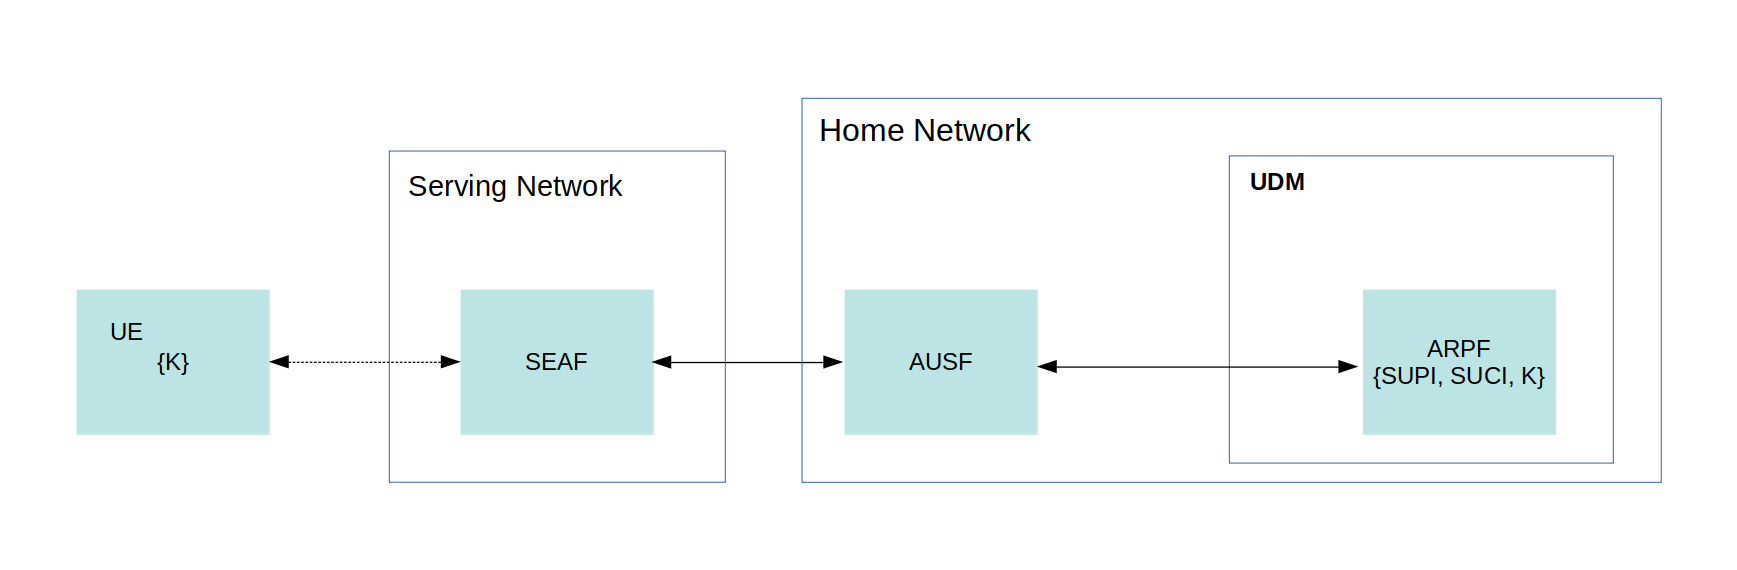
\includegraphics[scale=0.21]{Figure2_1.png}
	\end{center}
	\caption{Dashed lines indicate insecure connections.}
\end{figure}

Figure 2.1 gives a high level overview of the connections between the four components.
\newline

The protocol begins with an authorization request.  The request can be initiated by the UE or the SEAF.  Authentication can use either 5G-AKA or EAP-AKA protocol.  The 5G-AKA protocol provides proof of authentication to the home network while EAP-AKA does not.  

Assuming authentication is initiated by the UE, the UE sends a N1 message to the SEAF.  The message contains the UE's SUCI or 5G-GUTI.  The 5G-GUTI similar to the SUCI is a temporary identifier used by the UE for over air communications.  The SEAF sends a Nausf\textunderscore UEAuthentication\textunderscore Authenticate Request containing the UE SUCI or SUPI and the serving network name to the AUSF.  The AUSF temporarily stores the serving network name, and determines wether the network the request was received from has the right to use that name.  If the serving network name and the network the message was received from do not match, the authentication process is halted and a failure message is sent to the serving network.  If the SN name and the network the message is received from agree the AUSF passes the information from the SEAF on in an Nudm\textunderscore UEAuthentication\textunderscore Get Request to the ARPF.  The ARPF chooses whether EAP-AKA or 5G-AKA is used for authentication.  It also determines the SUPI of the UE if the SUCI was sent in the message.  

Up to this point the process is the same for EAP-AKA and 5G-AKA.  Once the determination is made which protocol to use, the two protocols diverge.  In 5G-AKA ARPF generates an authentication vector, for each Nudm\textunderscore UEAuthentication\textunderscore Get Request received.  The authentication vector consists of $<$RAND, AUTN, XRES*, $K_{ausf}$$>$.  The AUTN is the AUthentication TokeN.  And XRES* is the expected response from the UE.  The AV is returned to the AUSF in a Nudm\textunderscore UEAuthentication\textunderscore Get Response.  If the SUCI was included in the request the SUPI is included in the response.  Upon receipt the AUSF stores XRES* and the SUCI or SUPI temporarily.  

The AUSF generates HXRES* which is the SHA-256 hash of XRES*.  It generates $K_{seaf}$ from $K_{ausf}$.  XRES* is replaced by HXRES* and $K_{ausf}$ is replaced by $K_{seaf}$ inside the AV.  Before being sent in an Nausf\textunderscore UEAuthentication\textunderscore Authenticate Response to the SEAF, $K_{seaf}$ is removed from the AV.  Once received by the SEAF, the SEAF sends RAND, and AUTN to the UE in an Authentication Request message.  

The UE determines the freshness of the AV based off the AUTN.  If the AV is fresh, then it is accepted by the UE.  Using USIM, the UE computes a response, RES, CK, IK.  CK stands for cipher key.  IK stands for integrity key.  CK and IK are 128-bits and derived from K, the UE's permanent key, using RAND.  
\begin{quote}
	$CK = f_1(K||RAND) $ where $ f_1 $ is a key generating function.
	\newline
	$IK = f_2(K||RAND) $ where $ f_2 $ is a key generating function.
\end{quote} 
From RES, CK, and IK the UE computes $K_{ausf}$, $K_{seaf}$, and RES*.  The UE sends a NAS Authentication Response message to the SEAF containing RES*.  The SEAF computes the hash of RES* and compares it to the cached value, HRES*.  If the two are the same authentication is considered successful for the serving network.  The SEAF sends RES* and the SUPI or SUCI of the UE to AUSF in a Nausf\textunderscore UEAuthentication\textunderscore Authenticate Request.  

Upon receiving the Nausf\textunderscore UEAuthentication\textunderscore Authenticate Request the AUSF checks the freshness of the AV.  If the AV is considered stale, then from the point of view of the home network, authentication is considered a failure.  If the AV is fresh, RES* is compared to the cached value, XRES*, if the two are in agreement, authentication is considered successful for the home network.  The AUSF then sends a Nausf\textunderscore UEAuthentication\textunderscore Authenticate Response message back to the SEAF indicating the result of home network authentication.  If authentication was successful for the home network, the $K_{seaf}$ is included in the Nausf\textunderscore UEAuthentication\textunderscore Authenticate Response message.  If a SUCI or SUPI was included in the initiating message a SUPI is also included in the response.  No communication services are provided to the UE until the SEAF is given the UE SUPI.

\begin{figure}[h]
	\begin{center}
		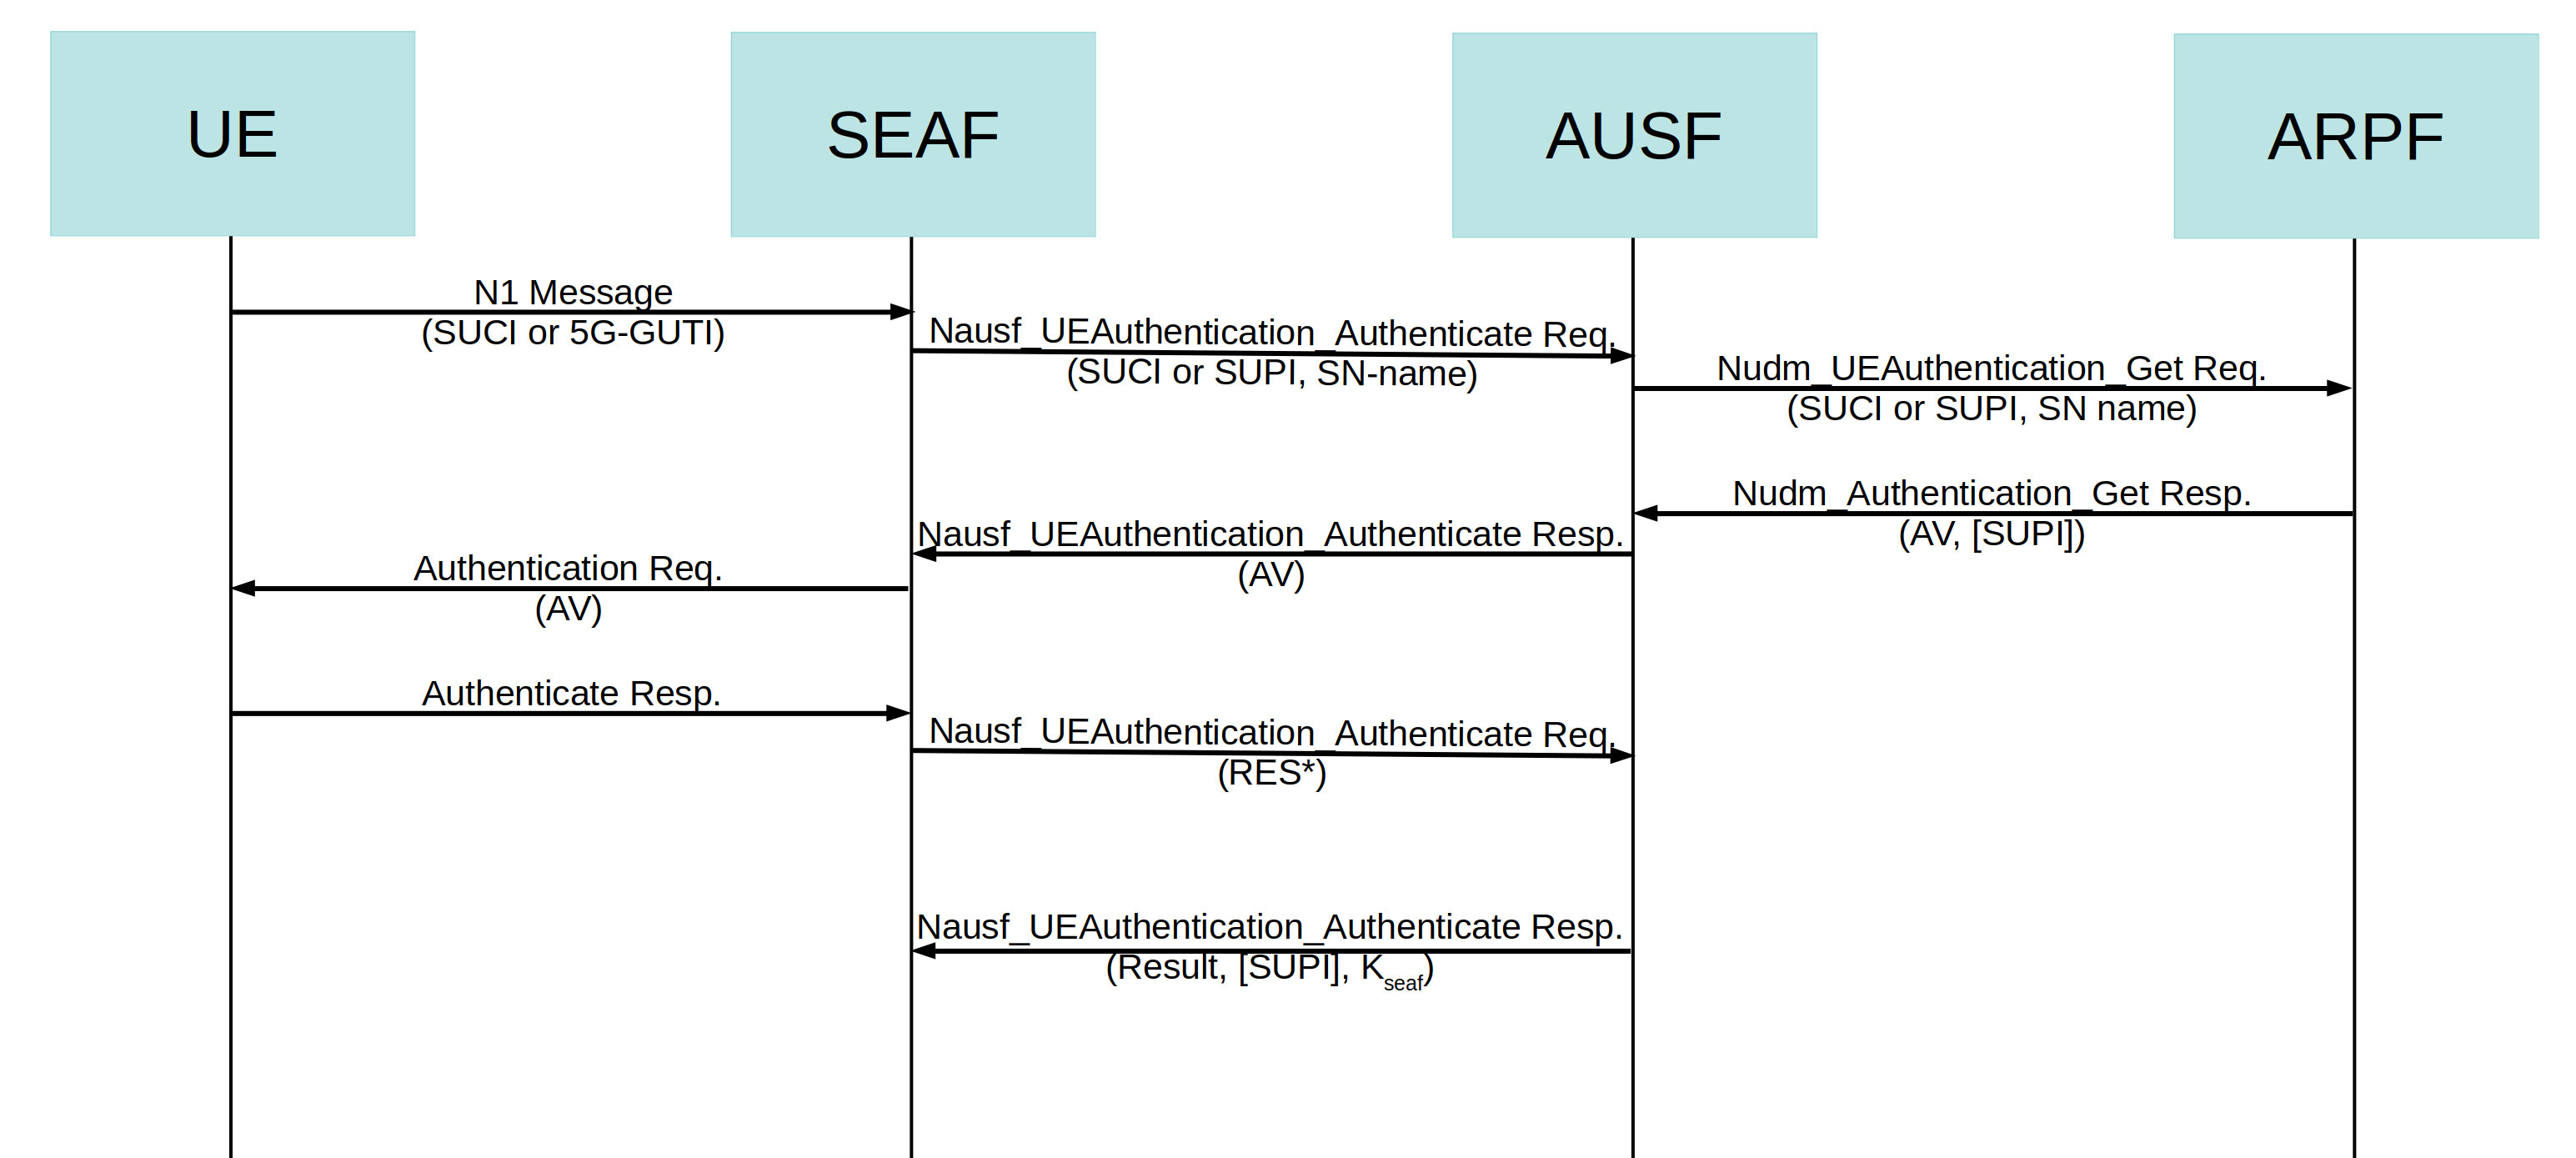
\includegraphics[scale=0.21]{Figure2_2.png}
	\end{center}
	\caption{5G-AKA protocol sequence diagram.}
\end{figure}


  









  

  

















\section{Related Work}
The Tamarin-Prover is software for the symbolic analysis and verification of security protocols.



     
\nocite{*}
\bibliography{References}
\bibliographystyle{plain}
\end{document}
